\documentclass[a4paper,12pt,french]{article}
\usepackage[margin=2cm]{geometry}
\usepackage[thinfonts]{uglix2}
\nouveaustyle

\begin{document}
\titre{Arbres binaires - Exercices}{NSI2}{2021} 

\begin{center}
\textit{Dans tout ce document, par arbre on entend arbre binaire.}
\end{center}

\begin{exercice}[: construire des arbres]
\begin{enumerate}[\bfseries 1.]
    \item   Dessiner tous les arbres binaires de taille 2.
    \item   Dessiner tous les arbres binaires de taille 3. 
\end{enumerate}
\end{exercice}


\begin{exercice}[: dénombrer des arbres]
Sachant qu'il existe
\begin{enumerate}[--]
    \item 1 arbre vide;
    \item 1 arbre de taille 1;
    \item 2 arbres de taille 2;
    \item 5 arbres de taille 3;
    \item 14 arbres de taille 5.
\end{enumerate}
Déterminer sans les construire le nombre d'arbres de taille 5.
\end{exercice}
\begin{exercice}[: une relation entre la hauteur et la taille d'un arbre]
Soit h un entier naturel et A un arbre de hauteur h.
\begin{enumerate}[\bfseries 1.]
    \item Combien, au minimum, A possède-t-il de n\oe uds ?
    \item Combien, au maximum, A possède-t-il de n\oe uds ?
\end{enumerate}

On en déduit l'encadrement suivant :\\
 soit N la taille d'un arbre de hauteur h, alors on a 
$$\Large\fbox{\hspace{3em}\leq N \leq\hspace{3em}}$$
\end{exercice}

\begin{exercice}[: Parcours \og à la main\fg{}]
    \begin{center}
        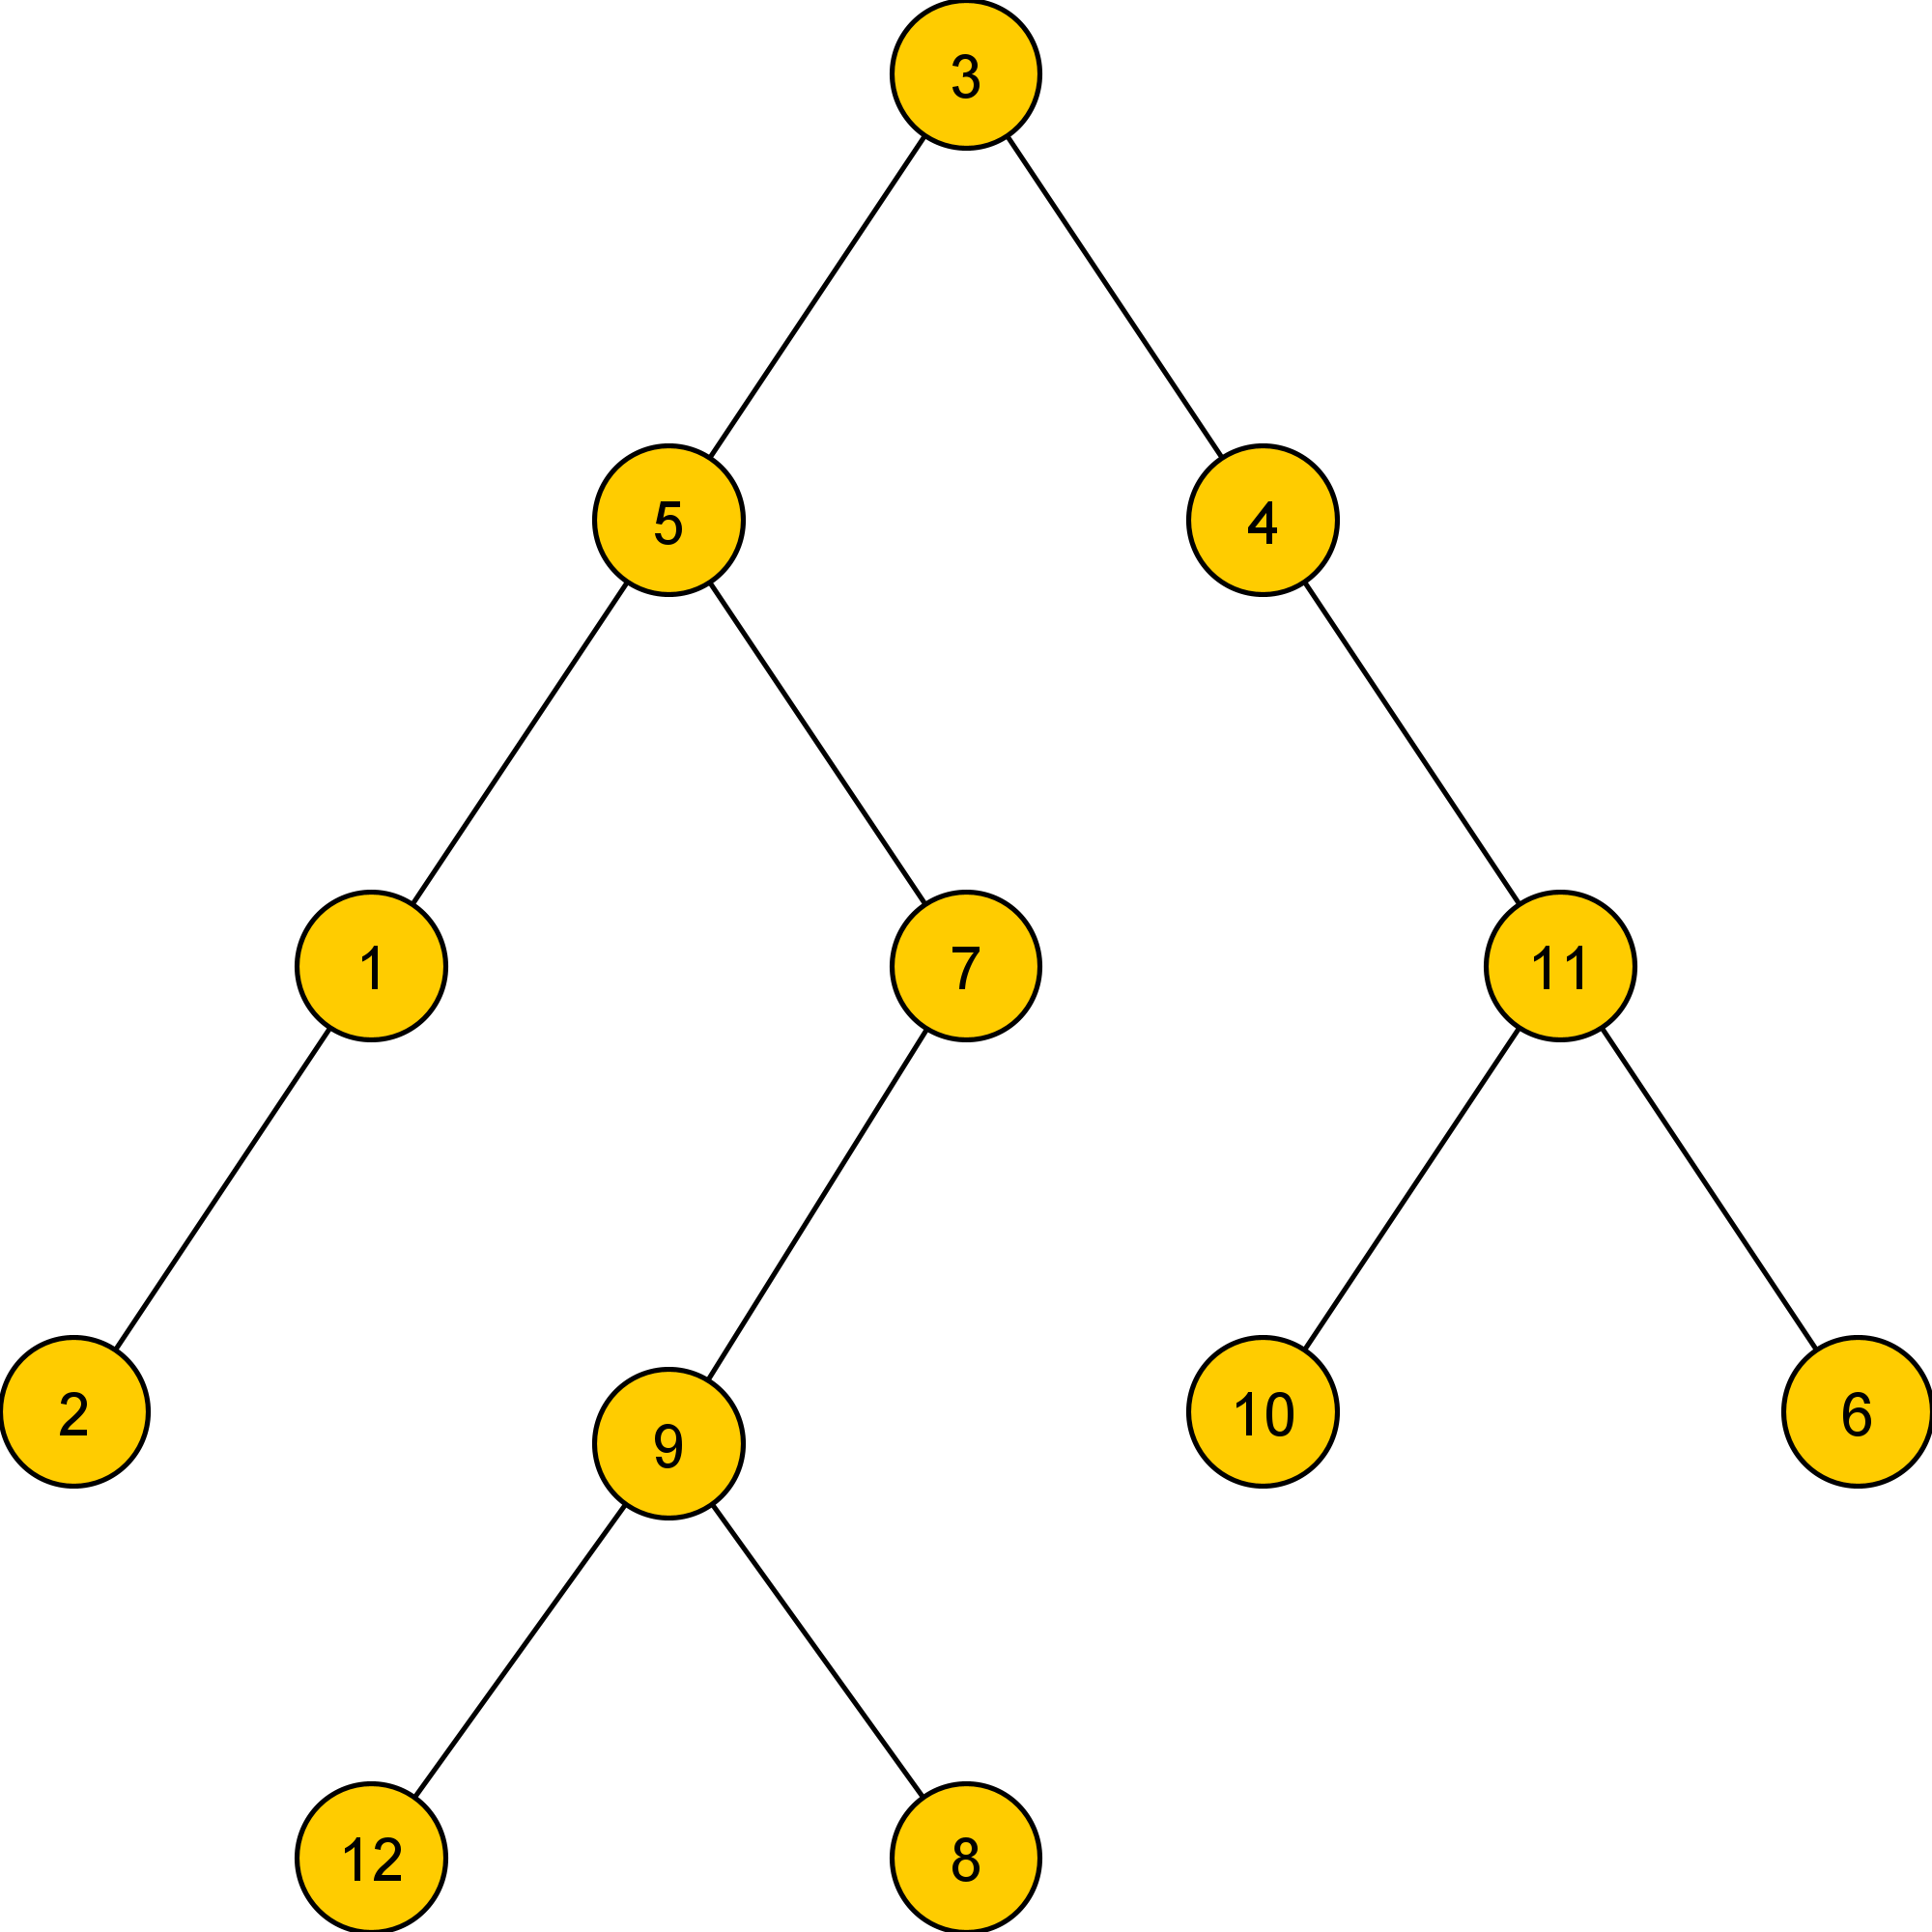
\includegraphics[width=7cm]{img/arbre2}
    \end{center}
\begin{enumerate}[\bfseries 1.]
    \item \'Ecrire les valeurs de l'arbre dans l'ordre de son parcours préfixe.
    \item Faire de même avec un parcours infixe.
    \item Faire de même avec un parcours postfixe.
\end{enumerate}
\end{exercice}

\begin{exercice}
    \begin{enumerate}[\bfseries 1.]
        \item Créer un fichier \texttt{Node.py} et implémenter la classe \texttt{Node} vue en cours.
        \item Implémenter la méthode \pythoninline{__str__} qui  utilise une sous-fonction récursive  qui :
        \begin{enumerate}[--]
            \item si on lui demande d'afficher \pythoninline{None} renvoie \pythoninline{''};
            \item sinon (c'est qu'elle doit bien afficher un n\oe ud)  ouvre une parenthèse, affiche récursivement le sous-arbre gauche, puis  affiche la valeur du n\oe ud, le sous-arbre droit et enfin ferme la parenthèse.\\
        \end{enumerate}
                      sur l'arbre suivant
    \begin{center}
        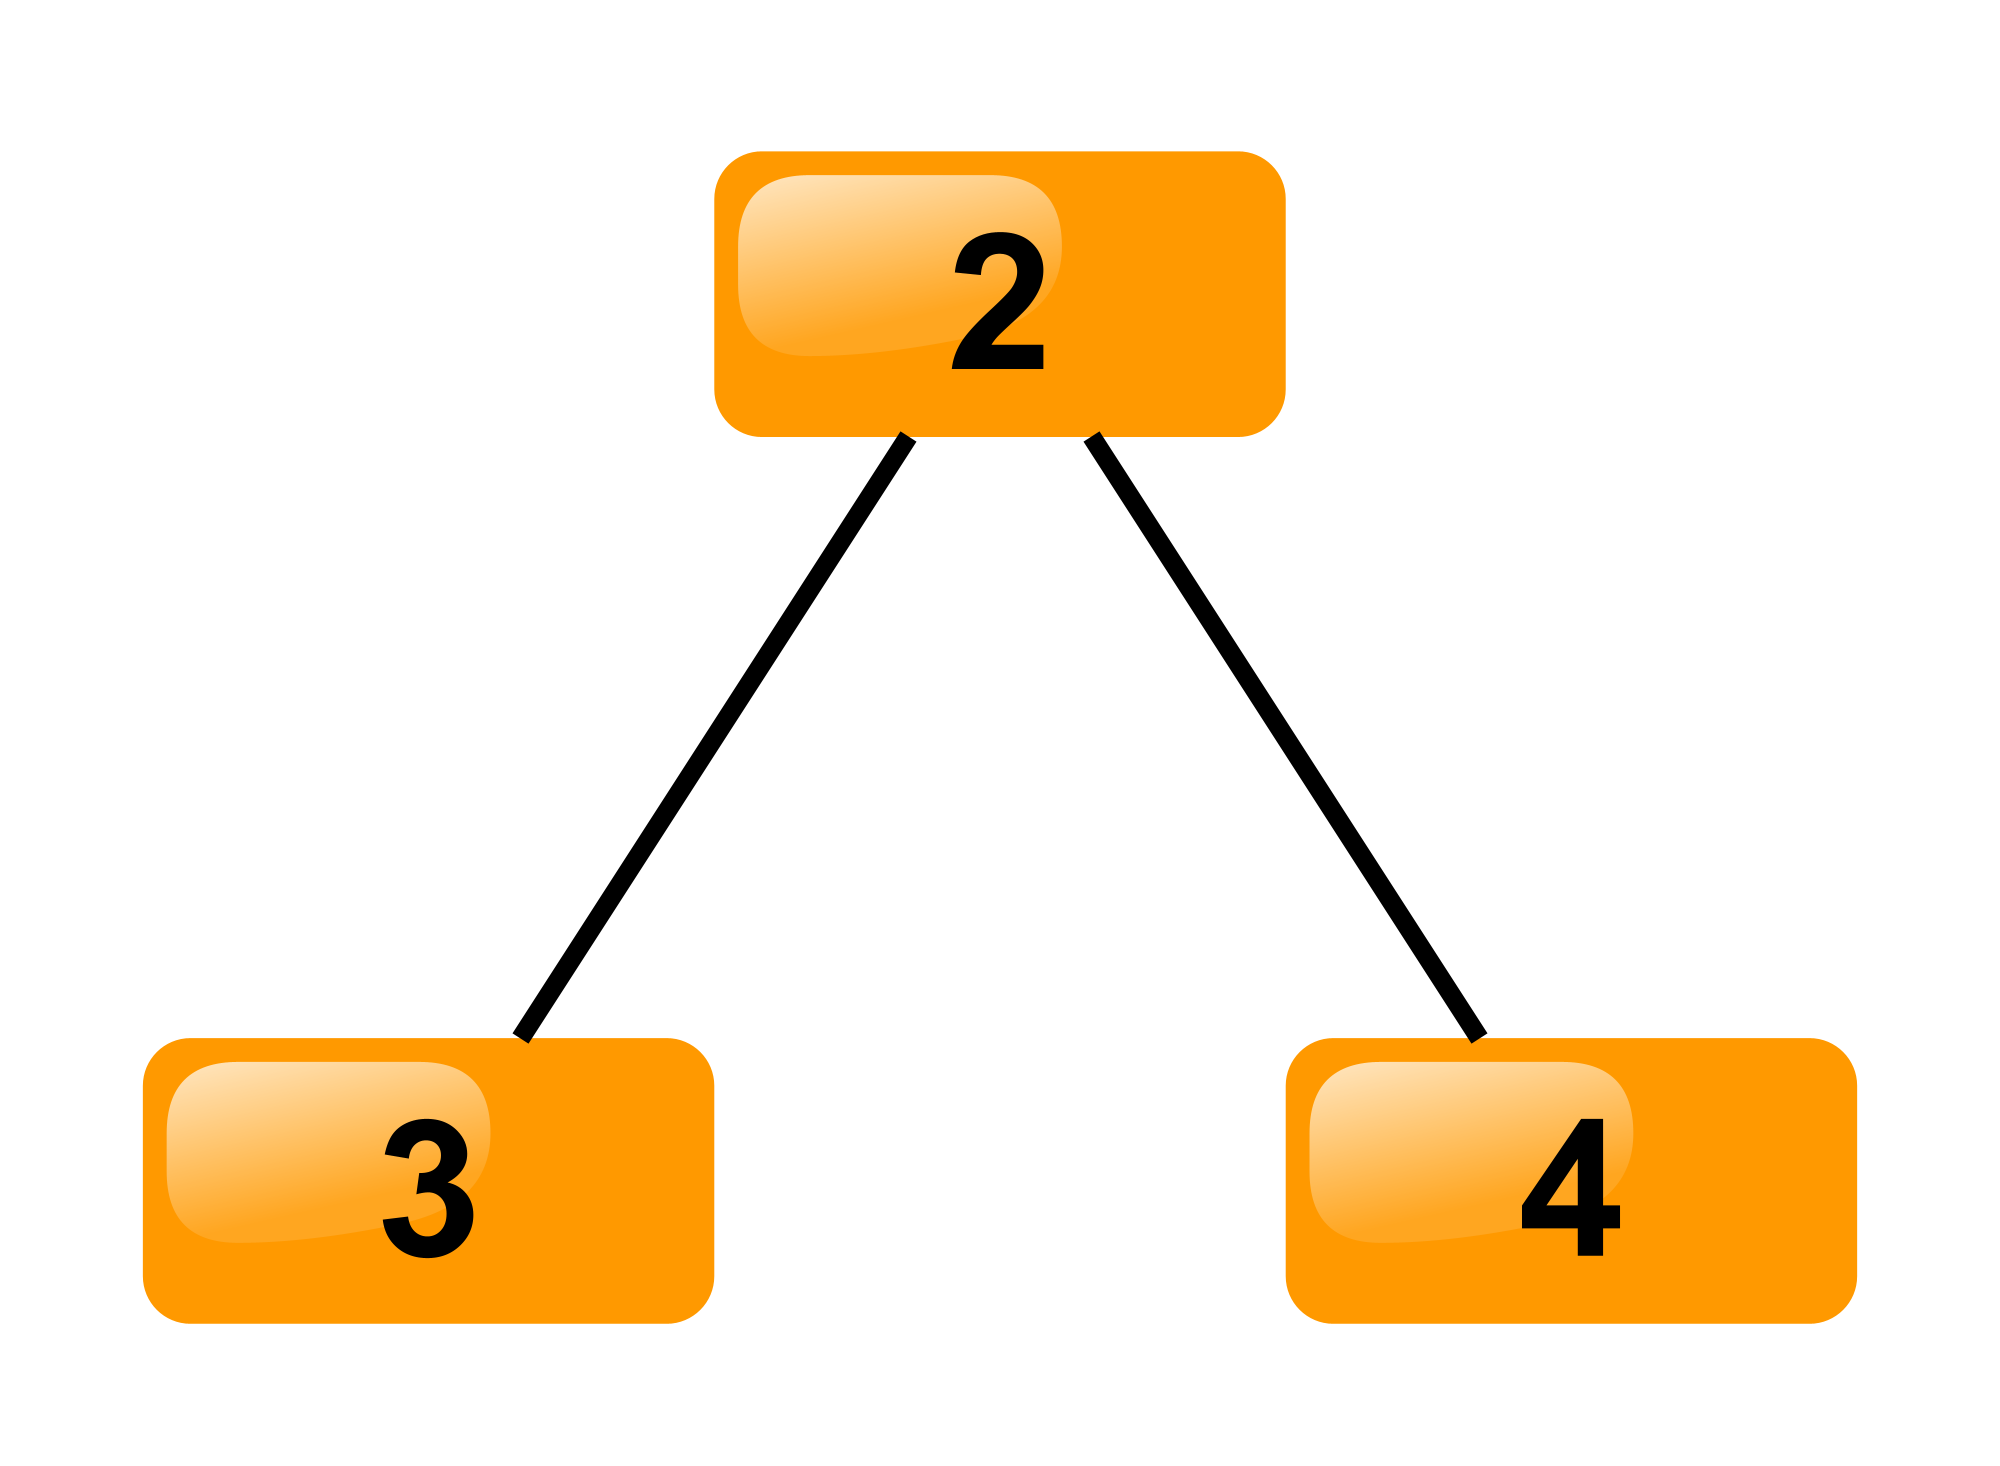
\includegraphics[width=3cm]{img/arbre1.png}
    \end{center}
    qui est créé par
\begin{minted}{python}
a = Node(3)
b = Node(4)
c = Node(2, a, b)
\end{minted}
    \pythoninline{print(c)} devra renvoyer \pythoninline{'((3)2(4))'}
\item Implémenter la méthode d'instance \pythoninline{size} qui renvoie un \pythoninline{int} qui est la taille de l'arbre (s'aider du cours).
\item Comment trouver récursivement la hauteur d'un arbre ? Proposer une \og méthode logique\fg{} et implémenter la méthode d'instance \pythoninline{height}, qui renvoie un \pythoninline{int} qui est la hauteur de l'arbre.
\item Implémenter la méthode d'instance \pythoninline{__eq__} qui renvoie \pythoninline{True} si deux arbres sont égaux et \pythoninline{False} sinon (trouver une méthode récursive).
    \end{enumerate}
\end{exercice}
\begin{exercice}[: Parcours]
\begin{enumerate}[\bfseries 1.]
    \item Ajouter à la classe \pythoninline{Node} une méthode d'instance \pythoninline{prefix} qui renvoie un \pythoninline{str} qui est la chaîne de caractères obtenue en concaténant toutes les valeurs des n\oe uds de l'arbre au cours de son parcours préfixe.
    \item De même implémenter \pythoninline{infix} et \pythoninline{postfix}.
\end{enumerate}
\end{exercice}
\end{document}